% Generated from data/synthetic_model_comparison/train/prompts_*/lion/001.txt.
% Verbatim prompt text, LaTeX-escaped only. Do not edit the prompt wording here.

\paragraph{The \texttt{compressed} prompt ($20$ words, $159$ characters)}
\begin{figure}[H]
\centering
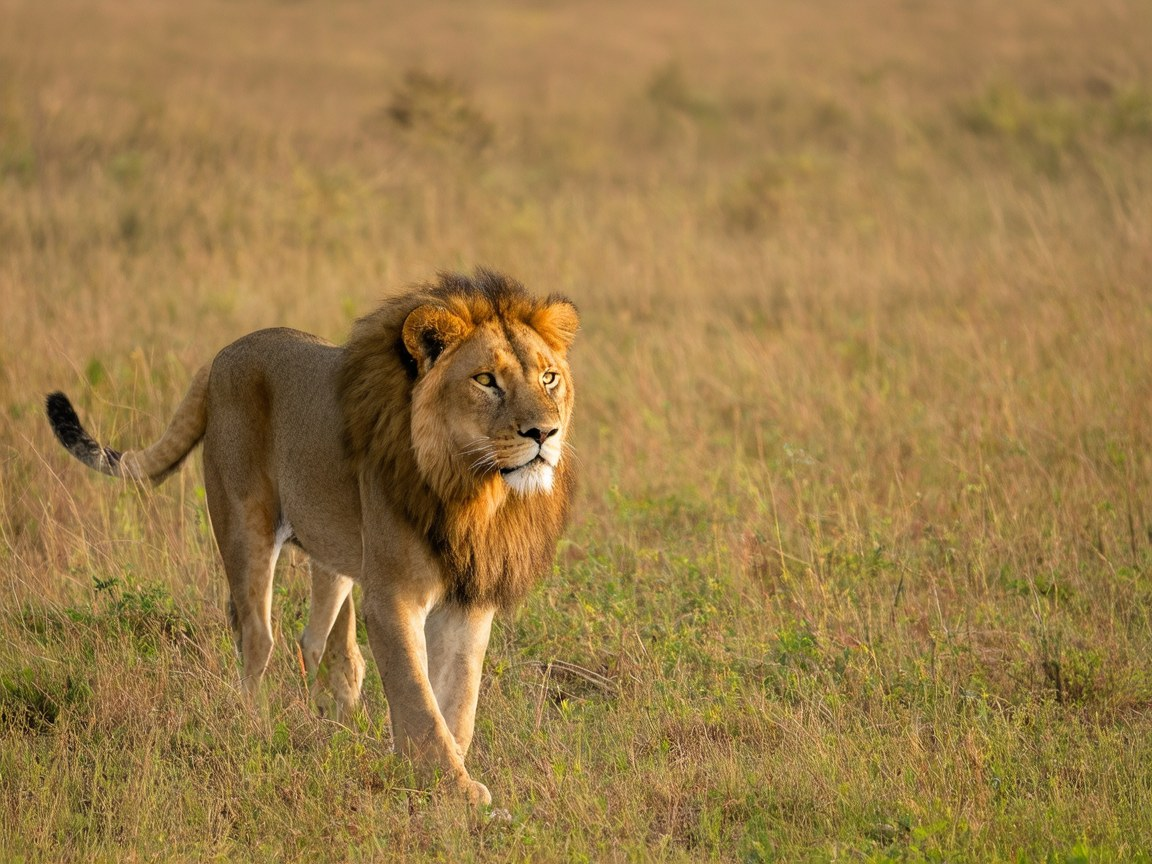
\includegraphics[width=0.48\textwidth]{figures/images/generator_comparison/appendix/lion_001_compressed_sd35m.jpg}
\caption{Lion slot $001$ rendered by SD 3.5 Medium from the \texttt{compressed} prompt below.}
\label{fig:appendix-prompt-slot-compressed}
\end{figure}
\begin{promptquote}
lion, tawny uniform coat, tufted tail, muscular shoulders, standing alert, on open savanna grassland, wildlife photograph, telephoto, photorealistic, full body
\end{promptquote}

\paragraph{The \texttt{maxlen} prompt, $256$-token tier ($149$ words, $963$ characters)}
\begin{figure}[H]
\centering
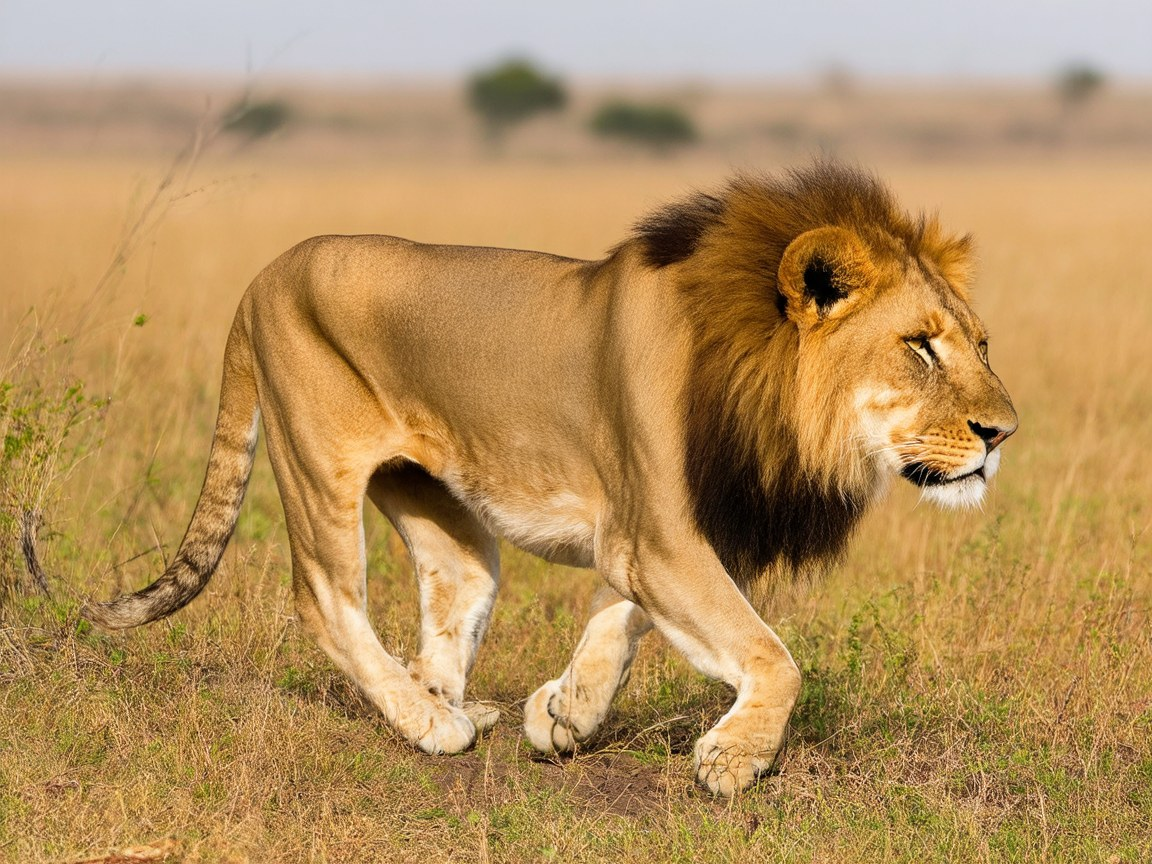
\includegraphics[width=0.48\textwidth]{figures/images/generator_comparison/appendix/lion_001_maxlen256_sd35m.jpg}
\caption{Lion slot $001$ rendered by SD 3.5 Medium from the $256$-token \texttt{maxlen} prompt below.}
\label{fig:appendix-prompt-slot-maxlen256}
\end{figure}
\begin{promptquote}
Realistic wildlife photograph of a lion (panthera leo). Species characteristics: tawny uniform coat, tufted tail, muscular shoulders. The lion is a muscular, broad-chested cat with a short, rounded head, a reduced neck, and round ears; males have broader heads. The fur varies in colour from light buff to silvery grey, yellowish red, and dark brown. The colours of the underparts are generally lighter. The lion trots along a game trail, its body fluid and powerful as it investigates a scent. A sun-bleached savanna with golden tall grass, scattered acacia trees, and a hazy background under a harsh midday sun. Professional wildlife photograph. Telephoto lens, sharp focus on the animal, natural lighting, photorealistic, high resolution. Full body of the animal visible, entire animal from head to tail fits within the frame. Natural habitat background. Exactly one lion in frame, diagnostic features clearly visible, no other individuals of the same species.
\end{promptquote}

\paragraph{The \texttt{maxlen} prompt, $512$-token tier ($380$ words, $2{,}264$ characters)}
\begin{figure}[H]
\centering
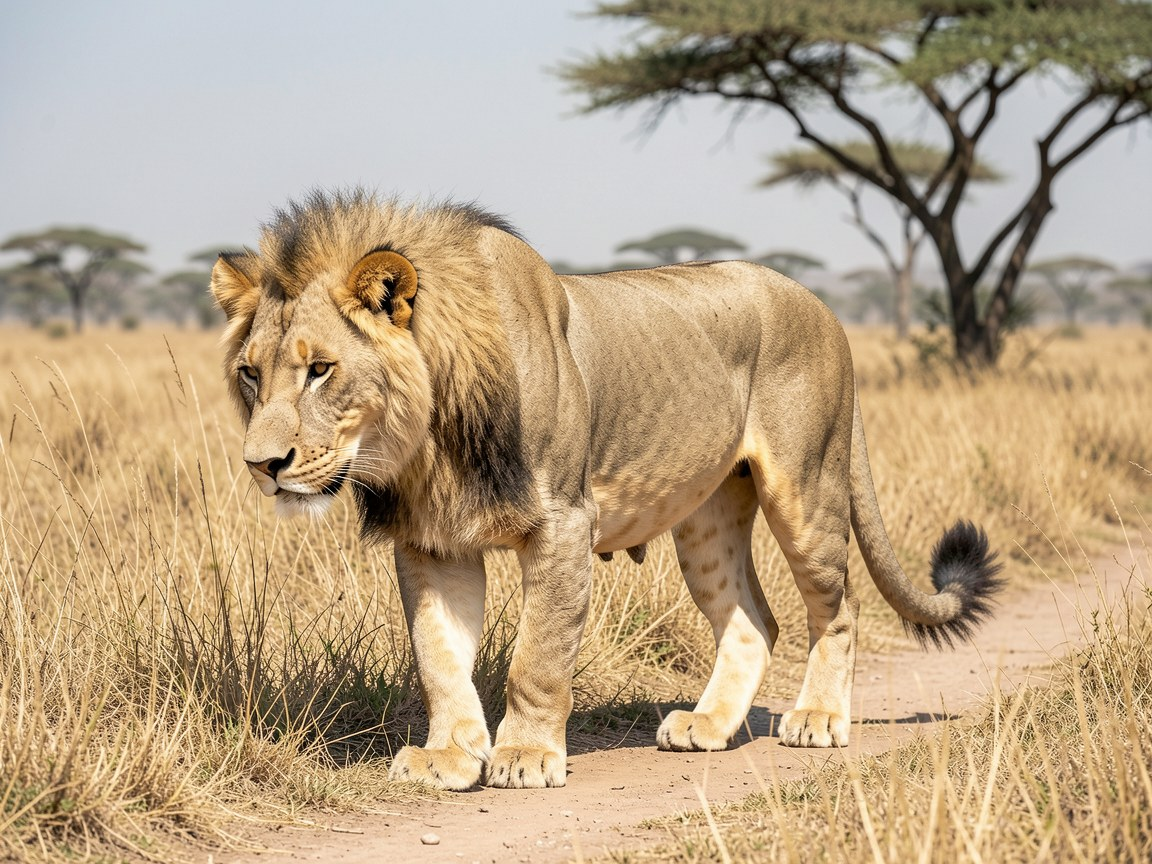
\includegraphics[width=0.48\textwidth]{figures/images/generator_comparison/appendix/lion_001_maxlen512_flux2-klein-9b.jpg}
\caption{Lion slot $001$ rendered by FLUX.2-klein from the $512$-token \texttt{maxlen} prompt below.}
\label{fig:appendix-prompt-slot-maxlen512}
\end{figure}
\begin{promptquote}
Realistic wildlife photograph of a lion (panthera leo). Species characteristics: tawny uniform coat, tufted tail, muscular shoulders. The lion is a muscular, broad-chested cat with a short, rounded head, a reduced neck, and round ears; males have broader heads. The fur varies in colour from light buff to silvery grey, yellowish red, and dark brown. The colours of the underparts are generally lighter. A newborn lion has dark spots, which fade as the cub reaches adulthood, although faint spots may still be seen on the legs and underparts. The tail of all lions ends in a dark, hairy tuft that, in some lions, conceals an approximately 5 mm (0.20 in)-long, hard \enquote{spine} or \enquote{spur} composed of dermal papillae. The functions of the spur are unknown. The tuft is absent at birth, develops at around 5+1/2 months of age, and is readily identifiable at the age of seven months. Its skull is very similar to that of the tiger. However, the frontal region is usually more depressed and flattened and has a slightly shorter postorbital region and broader nasal openings than those of the tiger. Due to the amount of skull variation in the two species, usually only the structure of the lower jaw can be used as a reliable indicator of species. The skeletal muscles of the lion make up 58.8\% of its body weight and represent the highest percentage of muscles among mammals. The lion has a high concentration of fast twitch muscle fibres, giving them quick bursts of speed but less stamina. Among felids, the lion is second only to the tiger in size. The size and weight of adult lions vary across their range and habitats. Accounts of a few individuals that were larger than average exist from Africa and Asia. The lion trots along a game trail, its body fluid and powerful as it investigates a scent. A sun-bleached savanna with golden tall grass, scattered acacia trees, and a hazy background under a harsh midday sun. Professional wildlife photograph. Telephoto lens, sharp focus on the animal, natural lighting, photorealistic, high resolution. Full body of the animal visible, entire animal from head to tail fits within the frame. Natural habitat background. Exactly one lion in frame, diagnostic features clearly visible, no other individuals of the same species.
\end{promptquote}

\paragraph{The \texttt{full} prompt ($4{,}642$ words, $28{,}032$ characters)}
\begin{figure}[H]
\centering
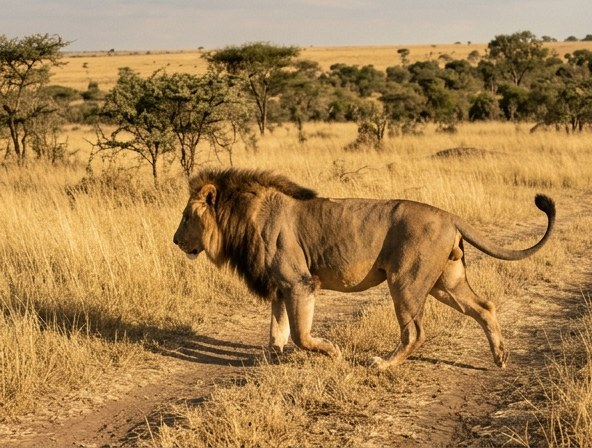
\includegraphics[width=0.48\textwidth]{figures/images/generator_comparison/appendix/lion_001_full_gemini.jpg}
\caption{Lion slot $001$ rendered by the production Gemini model from the \texttt{full} prompt below.}
\label{fig:appendix-prompt-slot-full}
\end{figure}
\begin{promptquote}
TASK: Generate a single photorealistic wildlife photograph for use in a computer vision object detection training dataset. The photograph must look like an authentic field photograph taken by a wildlife photographer or camera trap.

SUBJECT: lion (panthera leo)

SPECIES DESCRIPTION:

The lion is a muscular, broad-chested cat with a short, rounded head, a reduced neck, and round ears; males have broader heads. The fur varies in colour from light buff to silvery grey, yellowish red, and dark brown. The colours of the underparts are generally lighter. A newborn lion has dark spots, which fade as the cub reaches adulthood, although faint spots may still be seen on the legs and underparts. The tail of all lions ends in a dark, hairy tuft that, in some lions, conceals an approximately 5 mm (0.20 in)-long, hard \enquote{spine} or \enquote{spur} composed of dermal papillae. The functions of the spur are unknown. The tuft is absent at birth, develops at around 5+1/2 months of age, and is readily identifiable at the age of seven months.

Its skull is very similar to that of the tiger. However, the frontal region is usually more depressed and flattened and has a slightly shorter postorbital region and broader nasal openings than those of the tiger. Due to the amount of skull variation in the two species, usually only the structure of the lower jaw can be used as a reliable indicator of species.

The skeletal muscles of the lion make up 58.8\% of its body weight and represent the highest percentage of muscles among mammals. The lion has a high concentration of fast twitch muscle fibres, giving them quick bursts of speed but less stamina.

Among felids, the lion is second only to the tiger in size. The size and weight of adult lions vary across their range and habitats. Accounts of a few individuals that were larger than average exist from Africa and Asia.

The male lion's mane is the most recognisable feature of the species. It may have evolved around 320,000–190,000 years ago. It grows downwards and backward, covering most of the head, neck, shoulders, and chest. The mane is typically brownish and tinged with yellow, rust, and black hairs. Mutations in the genes microphthalmia-associated transcription factor and tyrosinase are possibly responsible for the colour of manes. It starts growing when lions enter adolescence, when testosterone levels increase, and reach their full size at around four years old. Cool ambient temperatures in European and North American zoos may result in a heavier mane. On average, Asiatic lions have sparser manes than African lions.

This feature likely evolved to signal the fitness of males to females. Males with darker manes appear to have greater reproductive success and are more likely to remain in a pride for longer. They have longer and thicker hair and higher testosterone levels, but they are also more vulnerable to heat stress. The core body temperature does apparently not increase regardless of sex, season, feeding time, length and colour of mane, but only surface temperature is affected. Unlike in other felid species, female lions consistently interact with multiple males at once. Another hypothesis suggests that the mane also serves to protect the neck in fights, but this is disputed. During fights, including those involving maneless females and adolescents, the neck is not targeted as much as the face, back, and hindquarters. Injured lions also begin to lose their manes.

Almost all male lions in Pendjari National Park are either maneless or have very short manes. Maneless lions have also been reported in Senegal, in Sudan's Dinder National Park and in Tsavo East National Park, Kenya. Castrated lions often have little to no mane because the removal of the gonads inhibits testosterone production. Lionesses rarely have manes. Increased testosterone may be the cause of maned lionesses reported in northern Botswana.

The white lion is a rare morph with a genetic condition called leucism, which is caused by a double recessive allele. It is not albino; it has normal pigmentation in the eyes and skin. White lions have occasionally been encountered in and around Kruger National Park and the adjacent Timbavati Private Game Reserve in eastern South Africa. They were removed from the wild in the 1970s, thus decreasing the white lion gene pool. Nevertheless, 17 births have been recorded in five prides between 2007 and 2015. White lions are selected for breeding in captivity. They have reportedly been bred in camps in South Africa for use as trophies to be killed during canned hunts.

NATURAL BEHAVIOR AND HABITAT:

Lions spend much of their time resting; they are inactive for about twenty hours per day. Although lions can be active at any time, their activity generally peaks after dusk with a period of socialising, grooming, and defecating. Intermittent bursts of activity continue until dawn, when hunting most often takes place. They spend an average of two hours a day walking and fifty minutes eating.

The lion is the most social of all wild felid species, living in groups of related individuals with their offspring. Such a group is called a \enquote{pride}. Groups of male lions are called \enquote{coalitions}. Females form the stable social unit in a pride and do not tolerate outside females. The majority of females remain in their birth prides while all males and some females disperse. The average pride consists of around 15 lions, including several adult females and up to four males and their cubs of both sexes. Large prides of up to 30 individuals have been observed. The sole exception to this pattern is the Tsavo lion pride that always had only one adult male. Prides act as fission–fusion societies, and members split into subgroups that keep in contact with roars.

Nomadic lions range widely and move around sporadically, either in pairs or alone. Pairs are more frequent among related males. A lion may switch lifestyles; nomads can become residents and vice versa. Interactions between prides and nomads tend to be hostile, although pride females in estrus allow nomadic males to approach them. Males spend years in a nomadic phase before gaining residence in a pride. A study undertaken in the Serengeti National Park revealed that nomadic coalitions gain residency at between 3.5 and 7.3 years of age. In Kruger National Park, dispersing male lions move more than 25 km (16 mi) away from their natal pride in search of their own territory. Female lions stay closer to their natal pride. Therefore, female lions in an area are more closely related to each other than male lions in the same area.

The evolution of sociability in lions was likely driven both by high population density and the clumped resources of savannah habitats. The larger the pride, the more high-quality territory they can defend; \enquote{hotspots} are near river confluences, where they have optimal access to water, prey, and vegetation cover. A study on three lion prides in a Zimbabwean wildlife reserve revealed that the dominant pride of 12 lions had the shortest average distance to water and the smallest home range of 130.35 km2 (50.33 sq mi); the smallest pride of four lions had the longest average distance to water and the largest home range of 174.6 km2 (67.4 sq mi).

The area occupied by a pride is called a \enquote{pride area,} whereas that occupied by a nomad is a \enquote{range}. Males associated with a pride patrol the fringes. Both males and females defend the pride against intruders, but the male lion is better-suited for this purpose due to its stockier, more powerful build. Some individuals consistently lead the defence against intruders, while others lag. Lions tend to assume specific roles in the pride; slower-moving individuals may provide other valuable services to the group. Alternatively, there may be rewards associated with being a leader that fends off intruders; the rank of lionesses in the pride is reflected in these responses. The male or males associated with the pride must defend their relationship with the pride from outside males who may attempt to usurp them.

Asiatic lion prides differ in group composition. Male Asiatic lions are solitary or associate with up to three males, forming a loose pride. In contrast, females associate with up to 12 other females, forming a greater pride together with their cubs. Female and male lions associate only when mating. Coalitions of males hold territory for a longer time than single lions. Males in coalitions of three or four individuals exhibit a pronounced hierarchy, in which one male dominates the others and mates more frequently.

The lion is a generalist hypercarnivore and is considered to be both an apex and keystone predator due to its wide prey spectrum. Its prey consists mainly of medium-sized to large hooved mammals, particularly blue wildebeest, plains zebra, African buffalo, gemsbok and giraffe. It also frequently takes common warthog despite it being much smaller. In India, chital and sambar deer are the most common wild prey, while livestock contributes significantly to lion kills outside protected areas. It usually avoids adult elephants, rhinoceros and hippopotamus and small prey like dik-dik, hyraxes, hares and monkeys, and seldom consumes other predators.

Young lions first display stalking behaviour at around three months of age, although they do not participate in hunting until they are almost a year old and begin to hunt effectively when nearing the age of two. Single lions are capable of bringing down zebra and wildebeest, while larger prey like buffalo and giraffe are riskier. In Chobe National Park, large prides have been observed hunting African bush elephants up to around 15 years old in exceptional cases, with the victims being calves, juveniles, and even subadults. In typical group hunts, each lioness has a favoured position in the group, either stalking prey on the \enquote{wing}, then attacking, or moving a smaller distance in the centre of the group and capturing prey fleeing from other lionesses. Males attached to prides do not usually participate in group hunting.

Some evidence suggests, however, that males are just as successful as females; they are typically solo hunters who ambush prey in small bushland. They frequently target large, less agile prey such as buffalo, and are also capable of hunting them solitarily. However, hunting in moderately sized coalitions yields higher success rates than operating alone or in overly large groups. Lions studied in Queen Elizabeth National Park increased their chances of success when hunting at night and moonless nights, when the prey was solitary and the cover of bushes dense; the chances of success increased when they attacked from a distance of 20 m (66 ft) and with a grass cover of 80 cm (31 in) tall.

Lions are not particularly known for their stamina. For instance, a lioness's heart comprises only 0.57\% of her body weight, and a male's is about 0.45\% of his body weight, whereas a hyena's heart comprises almost 1\% of its body weight. Thus, lions run quickly only in short bursts at about 48–59 km/h (30–37 mph) and need to be close to their prey before starting the attack. They take advantage of factors that reduce visibility; many kills take place near some form of cover or at night. One study in 2018 recorded a lion running at a top speed of 74.1 km/h (46.0 mph). Analysis of films of lion hunting has found that lions have an initial acceleration of 9.5 m/s2, while a Thomson's gazelle has an acceleration of only 4.5 m/s2, even though lions only would reach 50 km/h (31 mph) compared to the gazelles' nearly 97 km/h (60 mph); lions stalk their prey in order to attack them unexpectedly, as their prey begins to run unprepared while the predator is better prepared to start. The lion's attack is short and powerful; it attempts to catch prey with a fast rush and final leap, usually pulls it down by the rump, and kills with a clamping bite to the throat or muzzle. It can hold the prey's throat for up to 13 minutes, until the prey stops moving. A lioness has a bite force of 1593.8 Newtons (162.5 kgf) at the canine teeth.

Lions typically consume prey at the location of the hunt, but sometimes drag large prey into cover. They tend to squabble over kills, particularly the males. Cubs suffer most when food is scarce, but otherwise, all pride members eat their fill, including old and crippled lions, which can live on leftovers. Large kills are shared more widely among pride members. An adult lioness requires an average of about 5 kg (11 lb) of meat per day while males require about 7 kg (15 lb). Lions gorge themselves and eat up to 30 kg (66 lb) in one session. If it is unable to consume all of the kill, it rests for a few hours before continuing to eat. On hot days, the pride retreats to shade with one or two males standing guard. Lions defend their kills from scavengers such as vultures and hyenas.

Lions scavenge on carrion when the opportunity arises, scavenging animals dead from natural causes, such as disease, or those that other predators killed. Scavenging lions keep a constant lookout for circling vultures, which indicate the death or distress of an animal. Most carrion on which hyenas rather than lions kill both hyenas and lions feed. Carrion is thought to provide a large part of the lion's diet.

Lions and spotted hyenas occupy a similar ecological niche and compete for prey and carrion; a review of data across several studies indicates a dietary overlap of 58.6\%. Lions typically ignore hyenas unless they are on a kill or are being harassed, while the latter tend to visibly react to the presence of lions with or without the presence of food. In the Ngorongoro crater, lions subsist largely on kills stolen from hyenas, causing them to increase their kill rate. In Botswana's Chobe National Park, the situation is reversed as hyenas there frequently challenge lions and steal their kills, obtaining food from 63\% of all lion kills. When confronted on a kill, hyenas may either leave or wait patiently at a distance of 30–100 m (98–328 ft) until the lions have finished. Hyenas may feed alongside lions and force them off a kill. The two species attack one another even when there is no food involved for no apparent reason. Lions can account for up to 71\% of hyena deaths in Etosha National Park. Hyenas have adapted by frequently mobbing lions that enter their home ranges. When the lion population in Kenya's Masai Mara National Reserve declined, the spotted hyena population increased rapidly. Evidence of competition having a notable impact on either lion or spotted hyena populations was not found. In Tanzania's Ruaha-Rungwa, the spotted hyena population has increased with lion populations.

Lions tend to dominate cheetahs and leopards, steal their kills, and kill their cubs and even adults when given the chance. Cheetahs often lose their kills to lions or other predators. A study in the Serengeti ecosystem revealed that lions killed at least 17 of 125 cheetah cubs born between 1987 and 1990. Cheetahs avoid their competitors by hunting at different times and habitats. Nevertheless, cheetah population density remains stable, even when the lion population density increases. Leopards, by contrast, do not appear to be motivated by an avoidance of lions, as they use heavy vegetation regardless of whether lions are present in an area, and both cats are active around the same time of day. In addition, there is no evidence that lions affect leopard abundance. Leopards take refuge in trees, though lionesses occasionally attempt to climb up and retrieve their kills.

Lions similarly dominate African wild dogs, taking their kills and dispatching pups or adult dogs. Population densities of wild dogs are low in areas where lions are more abundant. However, there are a few reported cases of old and wounded lions falling prey to wild dogs.

Most lionesses reproduce by the time they are four years of age. Lions do not mate at a specific time of year, and the females are polyestrous. Like other cats, lions have penile spines that rake the walls of the vagina during copulation, which may cause ovulation. A lioness may mate with more than one male when she is in heat. Lions of both sexes may be involved in group homosexual and courtship activities. Males also head-rub and roll around with each other before mounting each other. Generation length of the lion is about seven years. The average gestation period is around 110 days; the female gives birth to a litter of between one and four cubs in a secluded den, which may be a thicket, a reed-bed, a cave, or some other sheltered area, usually away from the pride. She will often hunt alone while the cubs are still helpless, staying relatively close to the den. Lion cubs are born blind, their eyes opening around seven days after birth. They weigh 1.2–2.1 kg (2.6–4.6 lb) at birth and are almost helpless, beginning to crawl a day or two after birth and walking around three weeks of age. To avoid a buildup of scent attracting the attention of predators, the lioness moves her cubs to a new den site several times a month, carrying them one by one by the nape of the neck.

Lionesses of reproductive age within a pride have a similar number of surviving cubs, which they initially keep hidden. Lionesses without offspring do not assist in the care of the communal litter.

Usually, the mother does not integrate herself and her cubs back into the pride until the cubs are six to eight weeks old. Sometimes the introduction to pride life occurs earlier, particularly if other lionesses have given birth at about the same time. When first introduced to the rest of the pride, lion cubs lack confidence when confronted with adults other than their mother. They soon begin to immerse themselves in the pride life, however, playing among themselves or attempting to initiate play with the adults. Lionesses with cubs of their own are more likely to be tolerant of another lioness's cubs than lionesses without cubs. Male tolerance of the cubs varies—one male could patiently let the cubs play with his tail or his mane, while another may snarl and bat the cubs away.

Pride lionesses often synchronise their reproductive cycles and communal rearing and suckling of the young, which suckle indiscriminately from any or all of the nursing females in the pride. The synchronization of births is advantageous because the cubs grow to be roughly the same size and have an equal chance of survival, and older cubs do not dominate sucklings. Weaning occurs after six or seven months. Male lions reach maturity at about three years of age and at four to five years are capable of challenging and displacing adult males associated with another pride. They begin to age and weaken between 10 and 15 years of age at the latest.

When one or more new males oust the previous males associated with a pride, the victors often kill any existing young cubs, perhaps because females do not become fertile and receptive until their cubs mature or die. Females often fiercely defend their cubs from a usurping male, but are rarely successful unless a group of three or four mothers within a pride joins forces against the male. Cubs also die from starvation and abandonment, and predation by leopards, hyenas, and wild dogs. Male cubs are excluded from their maternal pride when they reach maturity at around two or three years of age, while some females may leave when they reach the age of two. When a new male lion takes over a pride, adolescents, both male and female, may be evicted.

Lions may live 12–17 years in the wild. Although adult lions have no natural predators, evidence suggests most die violently from attacks by humans or other lions. Lions often inflict serious injuries on members of other prides they encounter in territorial disputes or members of the home pride when fighting at a kill. Crippled lions and cubs may fall victim to hyenas and leopards or be trampled by buffalo or elephants. Careless lions may be maimed when hunting prey. Male lions may suffer more skull and teeth injuries when hunting very large prey than when fighting each other. Nile crocodiles also kill and eat lions, evidenced by the occasional lion claw found in crocodile stomachs.

Ticks commonly infest the ears, neck, and groin regions of lions. Adult forms of several tapeworm species of the genus Taenia have been isolated from lion intestines, having been ingested as larvae in antelope meat. Lions in the Ngorongoro Crater were afflicted by an outbreak of stable fly in 1962, resulting in lions becoming emaciated and covered in bloody, bare patches. Lions sought unsuccessfully to evade the biting flies by climbing trees or crawling into hyena burrows; many died or migrated, and the local population dropped from 70 to 15 individuals.

Captive lions have been infected with canine distemper virus since at least the mid-1970s. A 1994 outbreak in Serengeti National Park resulted in many lions developing neurological symptoms such as seizures, and several lions died from pneumonia and encephalitis. Feline immunodeficiency virus and lentivirus also affect captive lions.

When resting, lion socialisation occurs through a number of behaviours; the animal's expressive movements are highly developed. The most common peaceful, tactile gestures are head rubbing and social licking, which have been compared with the role of allogrooming among primates. Head rubbing, nuzzling the forehead, face, and neck against another lion appears to be a form of greeting and is seen often after an animal has been apart from others or after a fight or confrontation. Males tend to rub other males, while cubs and females rub females. Social licking often occurs in tandem with head rubbing; it is generally mutual, and the recipient appears to express pleasure. The head and neck are the most common parts of the body licked; this behaviour may have arisen out of utility because lions cannot lick these areas themselves.

Lions have an array of facial expressions and body postures that serve as visual gestures. A common facial expression is the \enquote{grimace face} or flehmen response, which a lion makes when sniffing chemical signals and involves an open mouth with bared teeth, raised muzzle, wrinkled nose, closed eyes, and relaxed ears. Lions also use chemical and visual marking; males spray urine and scrape plots of ground and objects within the territory.

The lion's repertoire of vocalisations is large; variations in intensity and pitch appear to be central to communication. Most lion vocalisations are variations of roaring, growling and snarling. Other sounds produced include puffing, humming, and exhalations similar to purring, while cubs communicate by meowing and bleating. Roaring is used to advertise the animal's presence. Lions most often roar at night, a sound that can be heard from a distance of 8 km (5.0 mi). A 2025 study identified four stages in a roaring sequence: moaning, full-roaring, intermediary roaring (which is shorter and deeper), and grunting.

African lions live in scattered populations across sub-Saharan Africa. The lion prefers grassy plains and savannahs, scrub bordering rivers, and open woodlands with bushes. It rarely enters closed forests. On Mount Elgon, the lion has been recorded up to an elevation of 3,600 m (11,800 ft) and close to the snow line on Mount Kenya. Savannahs with an annual rainfall of 300 to 1,500 mm (12 to 59 in) make up the majority of lion habitat in Africa, estimated at 3,390,821 km2 (1,309,203 sq mi) at most. Still, remnant populations are also present in tropical moist forests in West Africa and montane forests in East Africa. The Asiatic lion now survives only in and around Gir National Park in Gujarat, western India. Its habitat is a mixture of dry savannah forest and very dry, deciduous scrub forest.

In Africa, the range of the lion originally spanned most of the central African rainforest zone and the Sahara desert. In the 1960s, it became extinct in North Africa, except in the southern part of Sudan.

During the mid-Holocene, around 8,000-6,000 years ago, the range of lions expanded into Southeastern and Eastern Europe, partially re-occupying the range of the now extinct cave lion. In Hungary, the modern lion was present from about 4,500 to 3,200 years Before Present. In Ukraine, the modern lion was present from about 6,400 to 2,000 years Before Present. In Greece, it was common, as reported by Herodotus in 480 BC; it was considered rare by 300 BC and extirpated by AD 100.

In Asia, the lion once ranged in regions where climatic conditions supported an abundance of prey. It was present in the Caucasus until the 10th century. It lived in the Levant until the Middle Ages and in Southwest Asia until the late 19th century. By the late 19th century, it had been extirpated in most of Turkey. The last live lion in Iran was sighted in 1942, about 65 km (40 mi) northwest of Dezful, although the corpse of a lioness was found on the banks of the Karun river in Khuzestan province in 1944. It once ranged from Sind and Punjab in Pakistan to Bengal and the Narmada River in central India.

SCENE SPECIFICATION:

- Camera angle / perspective: Camera at the same height as the animal's mid-body, horizontal perspective. The animal's head orientation is NOT fixed to frontal; it may face in any direction (away from camera, in profile, or toward camera) as determined by the behavior description.

- Distance from subject: Standard field view — animal fills approximately 20–40\% of frame (\textasciitilde{}80–250 m telephoto)

- Animal pose / behavior: The lion trots along a game trail, its body fluid and powerful as it investigates a scent.

- Environment / background: A sun-bleached savanna with golden tall grass, scattered acacia trees, and a hazy background under a harsh midday sun.

- Lighting conditions: Warm directional golden-hour light, long shadows, rich warm tones

- Occlusion / visibility: Animal fully visible, no obstruction

- Special focus: Focus on the fluid transition of the shoulder muscles during movement and the correct proportion of the head to the body length. The retractable claw anatomy, coat texture, and the specific tuft of hair at the end of the tail are critical diagnostic features.

PHOTOGRAPHY STYLE: Documentary wildlife photography, comparable in quality and style to BBC Natural World or National Geographic. Wildlife observation through optical binoculars (8–10$\times$ magnification), full-scene sharp focus, authentic field conditions. No background blur — the animal is integrated into its environment, not isolated against a softened background. No studio lighting, no artificial backgrounds, no text overlays, no watermarks, no borders, no frames, no human-made objects unless contextually relevant to the scene.

CRITICAL REQUIREMENTS:

1. The lion must be the unmistakable primary subject of the photograph.

2. The following species-diagnostic features must be clearly visible and anatomically correct: tawny uniform coat, tufted tail, muscular shoulders, pronounced male mane, amber forward-facing eyes

3. The animal's body proportions, coloration, and posture must match the species description above exactly.

4. The scene must be ecologically plausible — the environment, weather, and behavior must all occur naturally for this species.

5. The photograph must be suitable for training an automated species identification system.

6. The animal must be fully visible within the frame — no part of its body, head, or limbs should be cut off at the image edges.

7. The animal's body and head orientation must match the angle specification and behavior description above exactly. Do not reorient the animal toward the camera to improve species feature visibility; instead render the diagnostic features from the specified angle.

8. Exactly one individual lion must appear in the photograph. No other individual of the same species should be clearly visible in the frame. Other species may appear incidentally in the distant background.
\end{promptquote}
